% ----------------------- TODO ---------------------------
%Template 
\documentclass[a4paper]{scrartcl}
\usepackage[utf8]{inputenc}
%\usepackage[ngerman]{babel}
\usepackage{geometry,forloop,fancyhdr,fancybox,lastpage, hyperref}
\usepackage{listings}
\lstset{frame=tb,
	language=Java,
	aboveskip=3mm,
	belowskip=3mm,
	showstringspaces=false,
	columns=flexible,
	basicstyle={\small\ttfamily},
	numbers=left,
	numberstyle=\tiny\color{gray},
	keywordstyle=\color{blue},
	commentstyle=\color{dkgreen},
	stringstyle=\color{mauve},
	breaklines=true,
	breakatwhitespace=true,
	tabsize=3
}
\geometry{a4paper,left=3cm, right=3cm, top=3cm, bottom=3cm}
% Diese Daten müssen pro Blatt angepasst werden:
\newcommand{\NUMBER}{4}
\newcommand{\EXERCISES}{3}
% Diese Daten müssen einmalig pro Vorlesung angepasst werden:
\newcommand{\COURSE}{Chip Design}
\newcommand{\TUTOR}{Julia Grosse}
\newcommand{\STUDENTA}{Stefan Wezel}
\newcommand{\STUDENTB}{Lukas Günthner}
%\newcommand{\STUDENTC}{Gwent Krause}
\newcommand{\DEADLINE}{\date}
% ----------------------- TODO ---------------------------



%Math
\usepackage{amsmath,amssymb,tabularx}

%Figures
\usepackage{graphicx,tikz,color,float}
\graphicspath{ {home/stefan/picures/} }
\usetikzlibrary{shapes,trees}

%Algorithms
\usepackage[ruled,linesnumbered]{algorithm2e}

%Kopf- und Fußzeile
\pagestyle {fancy}
\fancyhead[L]{Tutor: \TUTOR}
\fancyhead[C]{\COURSE}
\fancyhead[R]{\today}

\fancyfoot[L]{}
\fancyfoot[C]{}
\fancyfoot[R]{Seite \thepage}

%Formatierung der Überschrift, hier nichts ändern
\def\header#1#2{
	\begin{center}
		{\Large\bf Übungsblatt #1}\\
		{(Abgabetermin #2)}
	\end{center}
}

%Definition der Punktetabelle, hier nichts ändern
\newcounter{punktelistectr}
\newcounter{punkte}
\newcommand{\punkteliste}[2]{%
	\setcounter{punkte}{#2}%
	\addtocounter{punkte}{-#1}%
	\stepcounter{punkte}%<-- also punkte = m-n+1 = Anzahl Spalten[1]
	\begin{center}%
		\begin{tabularx}{\linewidth}[]{@{}*{\thepunkte}{>{\centering\arraybackslash} X|}@{}>{\centering\arraybackslash}X}
			\forloop{punktelistectr}{#1}{\value{punktelistectr} < #2 } %
			{%
				\thepunktelistectr &
			}
			#2 &  $\Sigma$ \\
			\hline
			\forloop{punktelistectr}{#1}{\value{punktelistectr} < #2 } %
			{%
				&
			} &\\
			\forloop{punktelistectr}{#1}{\value{punktelistectr} < #2 } %
			{%
				&
			} &\\
		\end{tabularx}
	\end{center}
}

\begin{document}
	
	\begin{tabularx}{\linewidth}{m{0.2 \linewidth}X}
		\begin{minipage}{\linewidth}
			\STUDENTA\\
			\STUDENTB\\
			%\STUDENTC
		\end{minipage} & \begin{minipage}{\linewidth}
			\punkteliste{1}{\EXERCISES}
		\end{minipage}\\
	\end{tabularx}
	
	%\header{Nr. \NUMBER}{\DEADLINE}
	
	% ----------------------- TODO ---------------------------
	% Hier werden die Aufgaben/Lösungen eingetragen:
	
	

\section*{Augabe 1:}
\subsection*{$1)$}
$t_{pges} = n \cdot A + B \sum_{i=1}^n \frac{w_{i+1}}{w_i}$\\
Werden alle Inverter-Weiten um den selben Faktor erhöht vergrößert sich die Laufzeit, da die Summe in der oben stehenden Formel größer wird.\\

\subsection*{$2)$}
Werden nur die weiten der vorhergehenden Inverter erhöht, wird die Summe in $t_{pges}$ kleiner, demnach wird auch die Verzögerungszeit kleiner.

\subsection*{$3)$}
$t_p = V_{dd} \cdot \frac{ C_a \cdot w_i + C_e \cdot w_{i+1}}{w_i \cdot K_t}$ mit $K_t$ ist konstante, abhängig von der verwendeten Technologie.\\
~\\
$\Rightarrow t_{pges} = \sum_{i=1}^{n} V_{dd} \cdot \frac{ C_a \cdot w_i + C_e \cdot w_{i+1}}{w_i \cdot K_t} = n\cdot \frac{V_{dd} \cdot C_A}{K_t} + \frac{V_{dd} \cdot C_E}{K_t} \cdot \sum_{i=1}^{n} \frac{w_{i+1}}{w_i}$\\
~\\
Wähle $A= \frac{V_{dd} \cdot C_A}{K_t}$ und $B =\frac{V_{dd} \cdot C_E}{K_t}$, da Konstant und jeweils abhängig von $V_{dd}$ und $K_t$.\\
~\\
$\Rightarrow t_{pges} = n \cdot A + B \cdot \sum_{i=1}^{n} \frac{w_{i+1}}{w_i} $


\section*{Aufgabe 3}
\subsection*{$a)$}
Schalter bzw. Relaiskontakt.

\subsection*{$b)$}
\begin{itemize}
	\item $I_1$ Invertiert die Eingänge für die TG's
	\item $I_2$ Sorgt dafür, dass wenn $a=1 \Rightarrow y=\overset{\_}{b}$
\end{itemize}

\subsection*{$c)$}
In dieser Schaltung kann es zu schwimmenden Ausgängen an den TG's kommen.\\
$T_1$ schwimmt für die Eingangsbelegung $a=1 \land b=0$ oder für $a=b=1$. $T_2$ schwimmt für $a=b=0$.\\
Dies sollte durch weitere Gatter oder entsprechenden Inverter mit PUN/PUD Schaltung umgangen werden.\\
Eine Möglichkeit wäre die hier gezeite Schaltung mit Pull-Up/Pull-Down Widerständen und einem nachgeschalteten ODER-Gatter. Die Widerstände sind äquivalent mit PUN/PDN Inverter Schaltungen austauschbar.\\

\begin{center}
	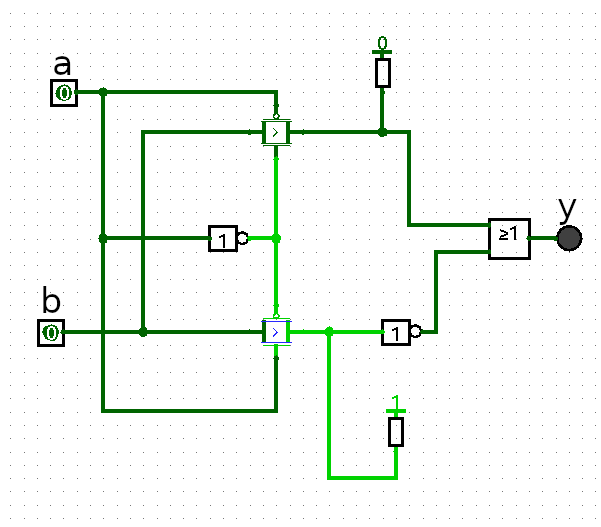
\includegraphics[width=0.7\textwidth]{b6_a3.png}	
\end{center}

\end{document}
